\subsection{Class Diagram}
This section will explain the most notable classes illustrated in \cref{fig:class} and its relations.

\subsubsection{Coordinate}
The \emph{Coordinate} trait models a geographic location on the earth. Because many functions are dealing with objects that can have coordinates, we can let these objects implement the \emph{Coordinate} trait, and thereby write these functions in a polymorphic way. One such object is the \emph{Position} class, which is essentially a coordinate for a person at a given time.

\emph{ConfidencePosition} is designed to have the same structure as positions received from the aSTEP server, so when hopMap request position data, a list of \emph{ConfidencePosition} will be returned. A \emph{ConfidencePosition} therefore also includes information about the certainty of a position, called \emph{Confidence} as shown on \cref{fig:class}. This confidence is the maximum distance a reading can be offset from the actual position of the device. \emph{ConfidencePosition} also has a \emph{lastLocatedTime} which is a time stamp for when the position was recorded by the aSTEP server.

\subsubsection{Person}
The \emph{Person} class is a abstract class, defining methods which should be implemented in specialisations of this class, in order to enforce code reuse and consistency. The class contains the person's history of positions as an iterateable collection of the generic type \emph{T}. 

The generic type parameter \emph{T} is bounded to be a class implementing \emph{Coordinate}, denoted by \emph{T < Coordinate}. This prevents any specialisation of \emph{Person} from having a history of positions that is not a collection of \emph{Coordinate}s. \emph{T} is in a contravariant position, denoted by \emph{-T}, permitting specialisations of the \emph{Person} class to use a specialisation of \emph{T}. Contravariance allows the \emph{Person} class to have methods that takes an input of type \emph{T}, but excludes the class from defining methods which returns a \emph{T}. 

The most important method in the \emph{Person} class is \emph{movePerson}, which takes a \emph{T} and a \emph{DateTime} as parameters. Here the parameter of type \emph{T} is the location the person should be moved to, and the DateTime parameter is the time where the person arrived at the location. This method updates a person's history of positions to include the new position. Upon updating a person's history of positions, positions older than \emph{x} is removed from the person, where \emph{x} is a constant defined for all persons. To calculate a person's velocity and heading direction this history of positions is essential.

\subsubsection{Area}
\emph{Area} is an abstract class representing a geographical area on a map. The most important method in the class that should implement is the function \emph{isWithinArea}. There are two versions of the function. One takes a coordinate and returns a boolean denoting weather this coordinate is within the area. The other takes a iterateable collection of generic types T and a function that goes from T to a coordinate. It returns a new filtered iterateable collection of T only consisting of the objects within the area.  

\subsubsection{PopulatedArea}
\emph{PopulatedArea} is a class mixing an area with a population. The responsibility of this class is to cache and update the positions of people within its area. The two main things this class must be able to do, is to update the positions of the people within it and be able to find the positions of all the people within it given a time. Since this is the class responsible for caching of peoples positions it also hold the policy of when to throw away positions and to extension the people holding them, if they for instance leave the area, and are no more relevant. It is therefore also responsible for any misses in its people position cache, and request the aSTEP for these positions. Since it is people themselves that throw away their positions this class must know about the policy of the person given to it, in order to be able to know when to request new positions from the aSTEP core and add these to the person. This class, together with the person class, hold the policy on how that given a specific time stamp, finding the position closest to this time stamp for each person, and judging when there is one close enough.

\alnote{Person[Position] og Person[ConfidencePosition] skal være abstract, og generalt check diagram}
\begin{sidewaysfigure}[htbp]
\centering
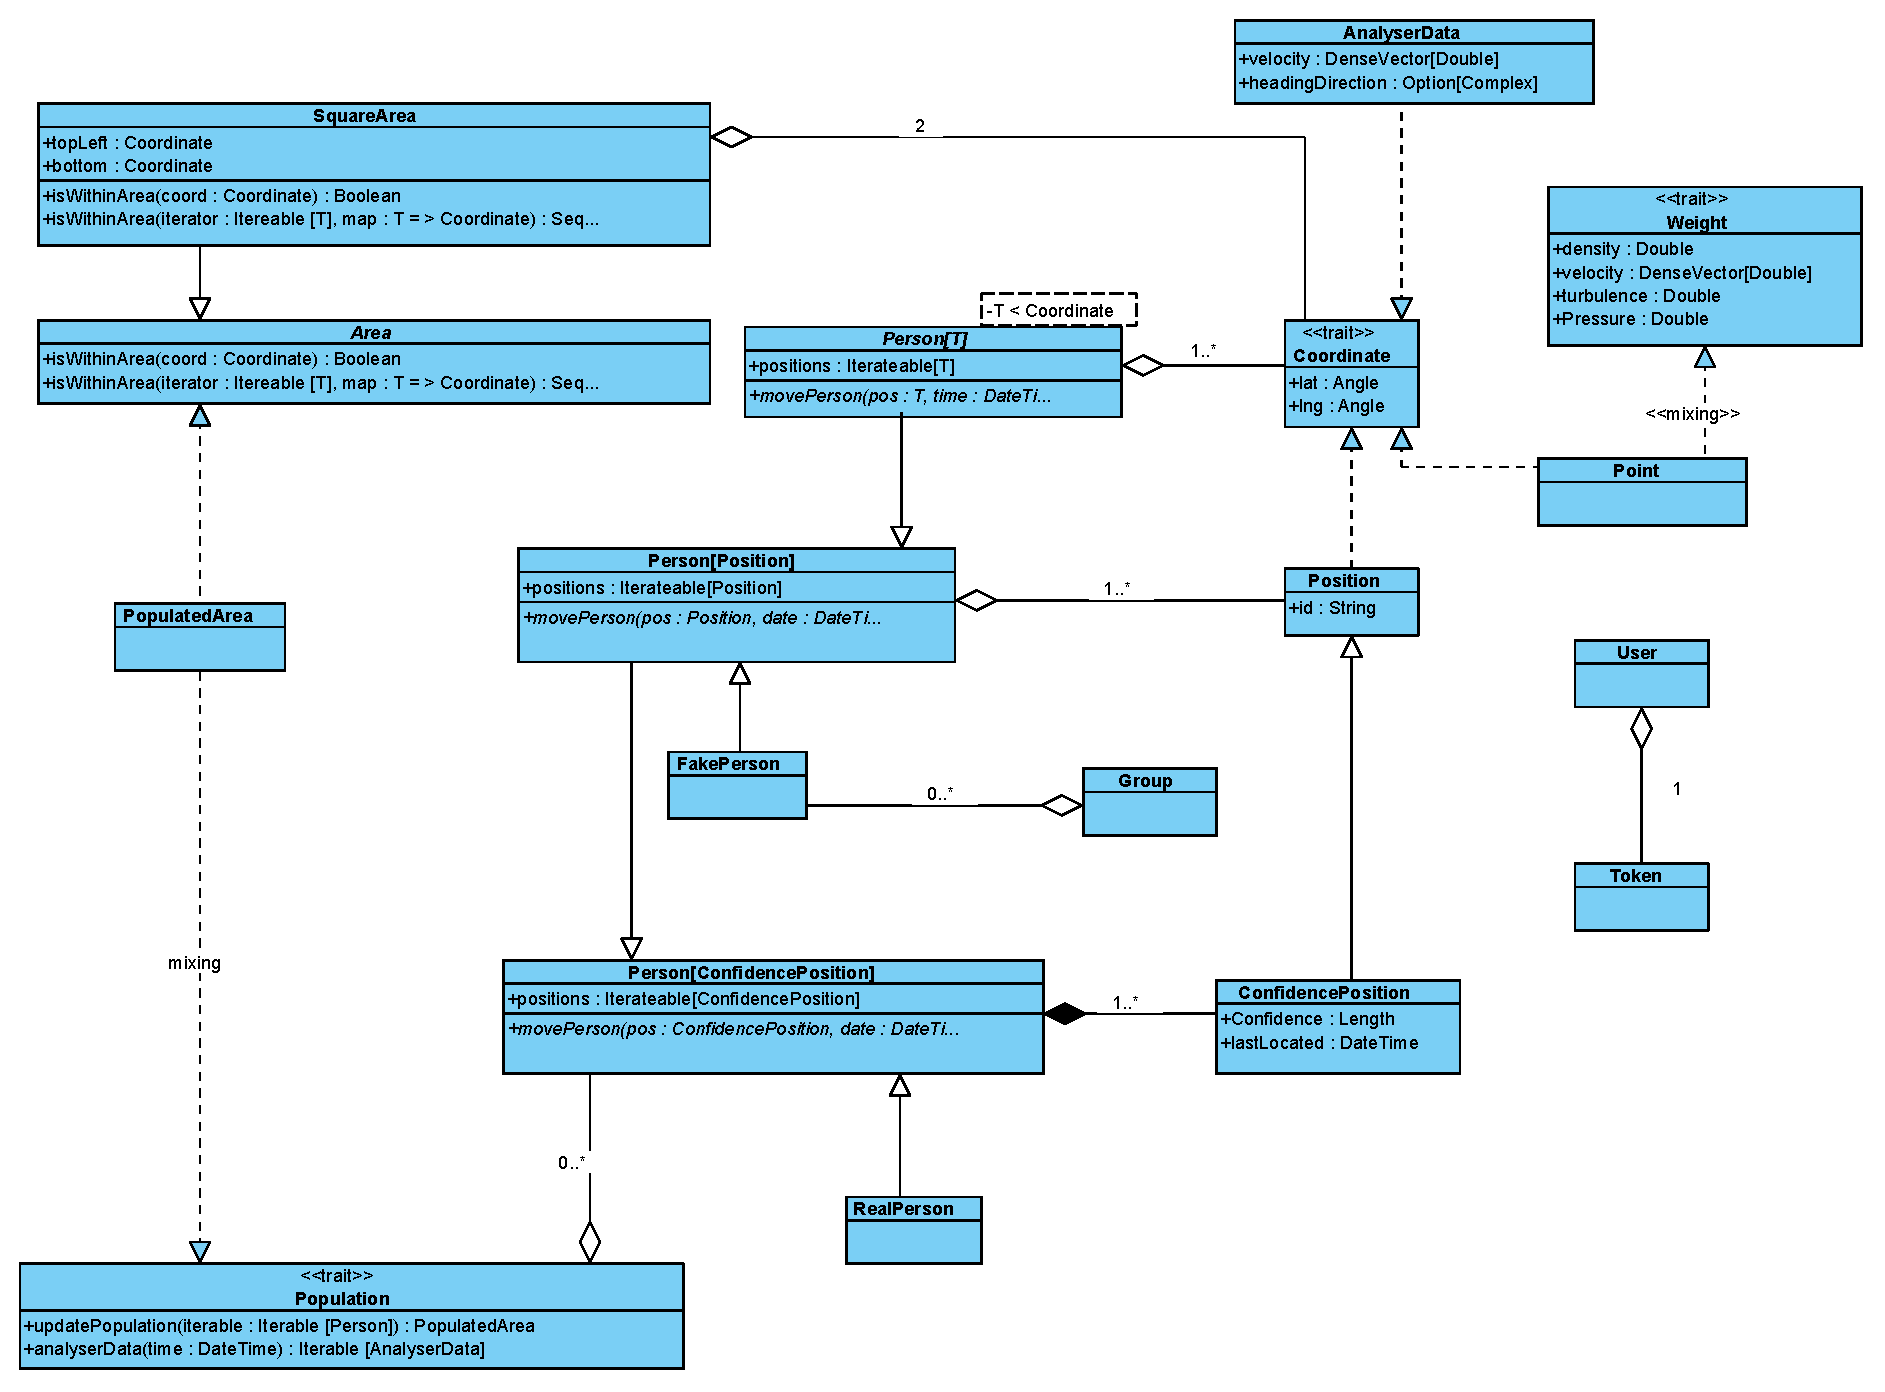
\includegraphics[width=\linewidth]{figures/class.eps}
\caption{Class diagram.}
\label{fig:class}
\end{sidewaysfigure}
